% XCircuit output "packet1.tex" for LaTeX input from packet1.eps
\def\putbox#1#2#3#4{\makebox[0in][l]{\makebox[#1][l]{}\raisebox{\baselineskip}[0in][0in]{\raisebox{#2}[0in][0in]{\scalebox{#3}{#4}}}}}
\def\rightbox#1{\makebox[0in][r]{#1}}
\def\centbox#1{\makebox[0in]{#1}}
\def\topbox#1{\raisebox{-0.60\baselineskip}[0in][0in]{#1}}
\def\midbox#1{\raisebox{-0.20\baselineskip}[0in][0in]{#1}}
   \scalebox{1}{
   \normalsize
   \parbox{7.78125in}{
   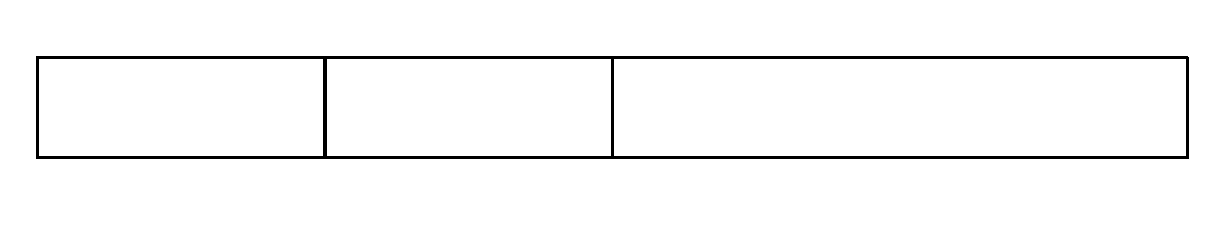
\includegraphics[scale=1]{packet1.eps}\\
   % translate x=976 y=150 scale 0.38
   \putbox{0.06in}{1.09in}{1.20}{31}%
   \putbox{1.97in}{1.09in}{1.20}{23}%
   \putbox{3.89in}{1.09in}{1.20}{15}%
   \putbox{7.72in}{1.09in}{1.20}{0}%
   \putbox{0.72in}{0.09in}{1.20}{length}%
   \putbox{2.64in}{0.09in}{1.20}{op-code}%
   \putbox{5.39in}{0.09in}{1.20}{command}%
   } % close 'parbox'
   } % close 'scalebox'
   \vspace{-\baselineskip} % this is not necessary, but looks better
